\section{Verificação e validação}
\subsection{Métodos de verificação}

\begin{frame}{Vulnerabilidades em CIs}
    \begin{block}{}
    Grande parte das vulnerabilidades encontradas em CIs escritos em Solidity poderiam ter sido evitadas com a ajuda de \textbf{análise formal} e \textbf{verificação} desses contratos antes de serem implantados na blockchain.
    \end{block}
    \begin{itemize}
        \item Linguagens como Solidity não foram desenvolvidas para serem verificadas formalmente;
        \item Solidity não é uma linguagem perfeita;
        \item Questões relacionadas com a execução dos CIs na Ethereum muitas vezes não são compreendidas pelos desenvolvedores.
    \end{itemize}
\end{frame}

\begin{frame}{Vulnerabilidades em CIs - Como evitar?}
    \textbf{Serviços de auditoria:}
    \begin{itemize}
        \item Organizações: OpenZeppeling, Solidified e SmartDec;
        \item Podem ser muito custosas para pequenas organizações e desenvolvedores autônomos.
    \end{itemize}
    \begin{exampleblock}{Solução}
    \textbf{Frameworks e ferramentas de verificação de CIs}
    \end{exampleblock}
\end{frame}

\begin{frame}{Verificação de CIs - Frameworks e ferramentas}
    Dois tipos de verificação:
    \begin{itemize}
        \item Proativa:
        \begin{itemize}
            \item Aplicada antes da implantação.
        \end{itemize}
        \item Reativa:
        \begin{itemize}
            \item Monitoramento do contrato durante a execução;
            \item Verificação em \textbf{tempo de execução}.
        \end{itemize}
    \end{itemize}
    Métodos de verificação:
    \begin{itemize}
        \item Análise de código;
        \item Métodos formais;
        \item \textit{Fuzzing};
        \item Técnicas de Inteligência Artificial (IA);
        \item Em tempo de execução.
    \end{itemize}
\end{frame}

\begin{frame}{Verificação de CIs - Análise de código}
    \begin{itemize}
        \item Estratégia geralmente automatizada;
        \item Detecção de erros;
        \item Identificação de vulnerabilidades;
        \item Aspectos analisados:
        \begin{itemize}
            \item Fluxo de controle;
            \item Fluxo de dados;
            \item Interface;
            \item Fluxo de informações;
            \item Caminhos de execução.
        \end{itemize}
        \item Verificação pode ser \textbf{estática}, \textbf{dinâmica} ou \textbf{híbrida};
        \item Normalmente é utilizada alguma representação intermediária estruturada:
        \begin{itemize}
            \item Grafo de fluxo de controle;
            \item Árvore sintática em XML.
        \end{itemize}
        \item \textbf{Execução simbólica}.
    \end{itemize}
\end{frame}

\begin{frame}{Verificação de CIs - Métodos formais}
    Modelagem formal de sistems:
    \begin{itemize}
        \item Representações matemáticas;
        \item Lógica de processos;
        \item Modelos baseados em estados;
        \item Especificação formal de propriedades;
        \item Verificação é realizada a partir das especificações fornecidas;
        \item Podem ser custosos em relação ao tempo e recursos;
        \item Aplicados em sistemas críticos.
    \end{itemize}
    Principais métodos:
    \begin{itemize}
        \item \textit{Model checking};
        \item Demonstração de teoremas;
        \item Verificação dedutiva.
    \end{itemize}
\end{frame}

\begin{frame}{\textit{Model checking}}
    \begin{itemize}
        \item Verificação de sistemas de transição de estados;
        \item Três etapas:
        \begin{itemize}
            \item Modelagem;
            \item Especificação: especificação formal dos requerimentos;
            \begin{itemize}
                \item Propriedades: Lógicas temporais.
            \end{itemize}
            \item Verificação.
        \end{itemize}
    \end{itemize}
    \begin{figure}[!htb]
     \centering
     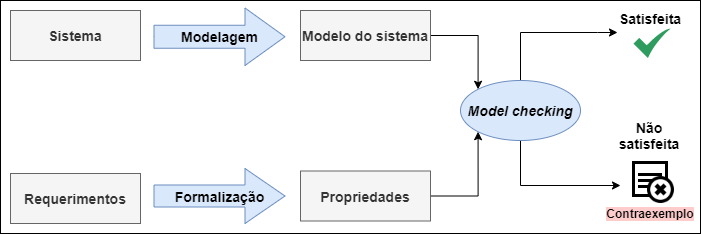
\includegraphics[scale=0.4]{figuras/verificacao/model-checking.png}
    \end{figure}    
\end{frame}

\begin{frame}{\textit{Model checking}}
    \begin{alertblock}{Problema: explosão de estados}
    Ocorre quando o modelo obtido a partir do código fornecido permite a exploração de uma quantidade excessivamente grande de estados.
    \end{alertblock}
    Alternativas:
    \begin{itemize}
        \item \textit{Model checking} simbólico;
        \item \textit{Model checking} limitado;
        \item \textit{Model checking} estatístico.
    \end{itemize}
\end{frame}

\begin{frame}{Métodos formais - Demonstração de teoremas}
    \begin{itemize}
        \item Modelagem do sistema e a especificação das propriedades é feita por meio de formalismos matemáticos;
        \item Uso de inferência dedutiva para produção de provas;
        \item Demonstrações são realizadas por meio de regras de inferência;
        \item Formalismos utilizados:
        \begin{itemize}
            \item Lógica proposicional;
            \item Lógica temporal;
            \item Lógica de ordem superior;
            \item Lógica de primeira ordem.
        \end{itemize}
    \end{itemize}
\end{frame}

\begin{frame}{Métodos formais - Verificação dedutiva}
\begin{itemize}
    \item Geração de provas matemáticas a partir do sistema e suas especificações;
    \item Se essas provas se mostrarem verdadeiras, então isso implica na conformidade do sistema com sua especificação.
\end{itemize}

\end{frame}

\begin{frame}{Verificação de CIs - \textit{Fuzzing}}
    \begin{itemize}
        \item Técnica para teste de software;
        \item \textit{Fuzzer}: Ferramenta para geração de entradas de teste de forma iterativa e aleatória;
        \item Baseado na geração de mutações de um conjunto de entradas;
        \item O \textit{fuzzer} encerra quando:
        \begin{itemize}
            \item Um objetivo é alcançado (ex: erro ou travamento do sistema);
            \item Tempo limite é atingido.
        \end{itemize}
    \end{itemize}
\end{frame}

\begin{frame}{Verificação de CIs - Inteligência artificial}
    \begin{itemize}
        \item \textbf{\textit{Machine learning}} e \textbf{\textit{deep learning}};
        \item CIs vulneráveis são convertidos em vetores ou matrizes;
        \item Modelos são utilizados para treinar os algoritmos;
        \item Em alguns casos, os modelos são obtidos com auxílio de outras ferramentas para verificação de CIs.
    \end{itemize}
\end{frame}

\begin{frame}{Verificação em tempo de execução}
    \begin{itemize}
        \item Código é instrumentalizado;
        \item É embutido um sistema de monitoramento;
        \item Assim, é possível reagir à atividades suspeitas;
        \item Violações de propriedades podem ser verificadas e prevenidas durante a execução do contratado;
        \item Método pouco utilizado.
    \end{itemize}
\end{frame}